% !TEX root = frenetic_programmers_guide.tex

\chapter{Gathering Statistics}
\label{chapter:statistics}

\section{Port Statistics}

Frenetic has two statistics-gathering mechanisms:

\begin{itemize}
\item The \netkat{port_stats} command gets per-port statistics.
\item The \netkat{SetQuery} policy gathers user-defined statistics.  You can use this in switch
policies or \netkat{pkt_out} actions, and aggregate them.
\end{itemize}

\begin{quotation}
\emph{SetQuery is not in the current Python bindings, but will be.  See Issue \#491 on Github}
\end{quotation}

\subsection{Modularizing Your Application}

We could add the statistics-gathering commands to an existing network application, like our learning
switch.  But Frenetic allows you more flexibility.   

We're going to write a completely separate application and run it as a separate process, but point it
at the same Frenetic instance as the learning switch.  The architecture looks something like this:

\begin{figure}[h]
\centering
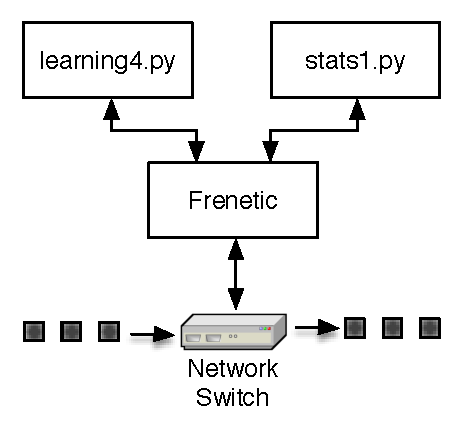
\includegraphics{dual_app_frenetic_architecture}
\end{figure}

This yields some nice advantages:

\begin{itemize}
\item We can combine the statistics application with other network applications.  It's like a 
library of network functions.
\item The resulting applications are much smaller, focused, and easy to understand and debug.
\item If the applications have large NetKAT policies, the process of separating them makes the 
updating them a bit faster.
\item If the applications are CPU intensive, you can run them on different servers or in different VM's.
\end{itemize}

One caveat is that all NetKAT policies from the applications are \netkat{Union}'ed together.  
Therefore, according
to NetKAT Principle 3, they should not have overlapping rules.  If this is a problem, you can use 
concerns to modularize your application instead, which we'll cover in Chapter \ref{chapter:modularization}.

The NIB for our statistics gathering process is fairly simple -- we save just the switch DPID and 
port list.  Although we could share the NIB with the other applications, keeping it separate frees us
from worrying about locks and so forth

The following code is in \codefilename{gathering_statistics/network_information_base.py}:

\inputminted{python}{code/gathering_statistics/network_information_base.py}

The statistics program itself doesn't need to send any NetKAT policies.  We set a 5 second timer,
and send the \netkat{port_stats} command each time, logging the response:

The following code is in \codefilename{gathering_statistics/stats1.py}:

\inputminted{python}{code/gathering_statistics/stats1.py}

Having started Mininet, Frenetic, and the Learning switch \codefilename{learning4.py} from Section 
\ref{l2_learning_switch:timeouts}, we can now start our app independently:

\begin{minted}{console}
vagrant@frenetic:~/manual/programmers_guide/code/gathering_statistics$ python stats1.py
Starting the tornado event loop (does not return).
2016-04-29 10:33:37,321 [INFO] Connected to Frenetic - Switches: {1: [4, 2, 1, 3]}
2016-04-29 10:33:42,333 [INFO] Count 1@3: {rx_bytes = 9590, tx_bytes = 10206}
2016-04-29 10:33:42,333 [INFO] Count 1@4: {rx_bytes = 8414, tx_bytes = 9100}
2016-04-29 10:33:42,334 [INFO] Count 1@2: {rx_bytes = 9562, tx_bytes = 10276}
2016-04-29 10:33:42,334 [INFO] Count 1@1: {rx_bytes = 10024, tx_bytes = 9184}
\end{minted}

Doing a \texttt{pingall} in the Mininet window will make the statistics go up.

What per-port statistics are available?  The following table gives you a list:

\begin{description}
\item[port\_no] Port number  
\item[rx\_packets] Number of packets received  
\item[tx\_packets] Number of packets transmitted  
\item[rx\_bytes] Number of bytes received  
\item[tx\_bytes] Number of bytes transmitted  
\item[rx\_dropped] Number of packets attempted to receive, but dropped  
\item[tx\_dropped] Number of packets attempted to transmit, but dropped
\item[rx\_errors] Number of packets errored upon receive 
\item[tx\_errors] Number of packets errored upon transmit
\item[rx\_fram\_err] Number of packets received with frame errors
\item[rx\_over\_err] Number of packets received with buffer overrun errors
\item[rx\_crc\_err] Number of packets received with CRC errors
\item[collisions] Number of collisions detected
\end{description}

These are the per-port statistics defined in OpenFlow 1.0.  

\section{Queries}

You can also gather statistics based on NetKAT rules.  This is called a \emph{query} and you can think 
of a query as just another location to send packets, like \netkat{SetPort} or \netkat{SetPipe}.
So Principle TODO applies here.  Recall that a packet can have only one destination: a port, a pipe or a 
query.  If you want packets to go to more than one destination, you need to use \netkat{Union} between
them so packet copies are made.

Unlike per-port statistics, a query only counts two things:

\begin{description}
\item[0] Number of packets  
\item[1] Number of bytes  
\end{description}

You call the \python{self.query()} command to get the current counts for this query at any time.

The following code is in \codefilename{gathering_statistics/stats2.py}:

\inputminted{python}{code/gathering_statistics/stats2.py}

So here, we set up a query called \python{"http"} and use it as a location to send packets.  The rule 
counts only HTTP requests initiated from port 1.  Every five minutes, we ask for a current count
from the query.  We can simulate an HTTP in Mininet like this:

\begin{minted}{console}
vagrant@frenetic:~$ sudo mn --topo=single,2 --controller=remote --mac
*** Creating network
*** Adding controller
Unable to contact the remote controller at 127.0.0.1:6633
*** Adding hosts:
h1 h2
*** Adding switches:
s1
*** Adding links:
(h1, s1) (h2, s1)
*** Configuring hosts
h1 h2
*** Starting controller
c0
*** Starting 1 switches
s1 ...
*** Starting CLI:
mininet> h2 python -m SimpleHTTPServer 80 &
mininet> h1 curl 10.0.0.2
<!DOCTYPE html PUBLIC "-//W3C//DTD HTML 3.2 Final//EN"><html>

 ... More output 
\end{minted}

And the output changes when the request is initiated:

\begin{minted}{console}
Starting the tornado event loop (does not return).
2016-05-11 14:51:46,565 [INFO] Connected to Frenetic - Switches: {1: [2, 4, 1, 3]}
2016-05-11 14:52:06,572 [INFO] Count: {packets = 0, bytes = 0}
2016-05-11 14:52:11,571 [INFO] Count: {packets = 0, bytes = 0}
2016-05-11 14:58:18,802 [INFO] Count: {packets = 11, bytes = 806}
2016-05-11 14:58:23,802 [INFO] Count: {packets = 11, bytes = 806}
\end{minted}
